\lecturetitle{\course}{ISO/IEC 15504 ou SPICE}

\frame{\maketitle}

\section{SPICE}

\begin{frame}{O que é SPICE?}
  \begin{itemize}[<+->]\setbeamercovered{transparent}
  \item {\bf SPICE}--{\em Software Process Improvement and Capability dEtermination}
    \begin{itemize}[<+->]\setbeamercovered{transparent}
    \item Norma ISO/IEC ({\em \href{International Electrotechnical
          Commission}{International Organization for
          Standardization}/\href{http://www.iec.ch/}{International
          Electrotechnical Commission}})
      \href{https://pt.wikipedia.org/wiki/ISO/IEC_15504}{15504} para
      avaliação de processos de construção de software.
    \item Derivada inicialmente da norma para ciclo de vida do
      processo ISO 12207 e de outros modelos de maturidade como
      Bootstrap, Trillium e CMM ({\em Capability Maturity Model}).
    \item Usada principalmente na industria automobilística da Europa e Austrália.
    \end{itemize}
  \item Objetivo: Fornecer modelos de avaliações que possam ser
    objetivas, reproduzidas e comparáveis.
  \end{itemize}  
\end{frame}

\begin{frame}{Objetivo das Avaliações}
  \begin{columns}
    \begin{column}{.3\textwidth}
      \includegraphics[scale=.4]{spice-assess.png}      
    \end{column}
    \begin{column}{.7\textwidth}
      \begin{itemize}[<+->]\setbeamercovered{transparent}
      \item O objetivo da avaliação é fazer com que o processo 
        atinja um alto grau de capacitação se aliando ao 
        objetivo do negócio.
      \item Avaliações permitem fornecer subsídios para os aperfeiçoamentos, 
        bem como detectar os pontos fracos e fortes do processo.
      \end{itemize}
    \end{column}
  \end{columns}
\end{frame}

\begin{frame}{SPICE}{Histórico}
   \begin{description}[<+->]\setbeamercovered{transparent}
  \item[1991] ISO/IEC aprovaram um estudo para investigar as necessidades 
    e requisitos para uma norma de avaliação de software.
  \item[1993] O Projeto SPICE foi iniciado com o objetivo de:
    \begin{itemize}[<+->]\setbeamercovered{transparent}
    \item Dar suporte ao desenvolvimento inicial de propostas;
    \item Implantar testes para ganho de experiência prévia;
    \item Conscientizar os usuários.
    \end{itemize}
  \item[1995] Início dos testes com os usuários e avaliação de propostas.
  \item[1995] Primeiro conjunto de propostas formando a base de um relatório 
    técnico.
  \item[1999--2003] Conversão em Norma ISO/IEC 15504.
  \end{description}
\end{frame}

\begin{frame}{Estrutura do modelo SPICE}
  O modelo de referencia de avaliação eh bidimensional:
  \begin{itemize}[<+->]\setbeamercovered{transparent}
  \item {\bf Dimensão do processo:} contem o processo em grupos;
  \item {\bf Dimensão da capacidade do processo:} permite que a capacidade 
    de cada processo seja medida de forma independente.
  \end{itemize}
\end{frame}

\subsection{A Dimensão do Processo}

\frame{\date{}\author{}\title{A Dimensão do Processo}\maketitle}

% \begin{frame}{SPICE}{Conceitos}\small
  
%   O modelo de arquitetura SPICE contem cinco categorias de processos descritas 
%   a seguir com a sigla em inglês entre parênteses:
  
%   \begin{description}[<+->]\setbeamercovered{transparent}
%   \item[Cliente-Fornecedor (CUS):] ({\em CUstomer-Supplier}) processos que afetam diretamente o
%     cliente, suporte à implantação do software, suporte à
%     orientação para o uso correto.
%   \item[Engenharia (ENG):] ({\em ENGineering}) processos que diretamente especificam, implementam 
%     ou mantêm um software e sistema e seu manual de usuário.
%   \item[Apoio (SUP):] ({\em SUPport}) processos que dão suporte à melhoria de performance 
%     de outros processos.
%   \item[Gestão (MAN):] ({\em MANagement}) processos que estabelecem o projeto e gerenciam
%     seus recursos.
%   \item[Organizacional (ORG):] ({\em ORGanization}) processos que estabelecem os objetivos dos 
%     negócios da organização e desenvolvem os recursos necessários para 
%     a divulgação do produto.
%   \end{description}

% \end{frame}

\begin{frame}{Modelo de referência dos processos}
O modelo de referência agrupa os processos em 3 categorias:

\begin{enumerate}[<+->]\setbeamercovered{transparent}
\item Ciclo de vida primário
\item Ciclo de vida de suporte
\item Ciclo de vida organizacional
\end{enumerate}

\pause\bigskip
Dentro das categorias os processos são agrupados em um segundo nível
de acordo com o tipo de atividade.
\end{frame}


\begin{frame}{Modelo de Referência SPICE}
  
  \begin{center}
    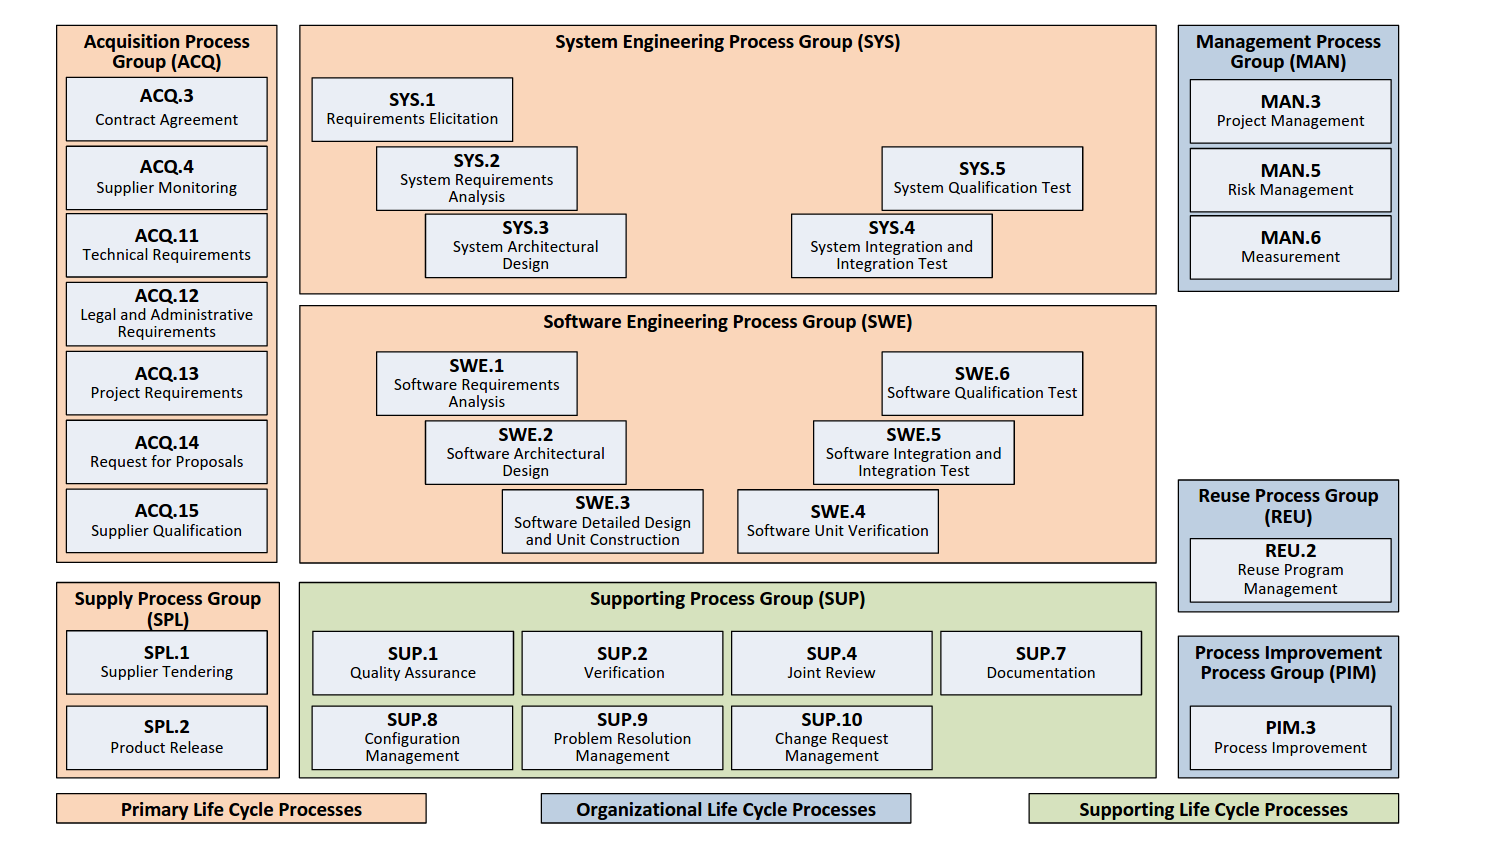
\includegraphics[scale=.237]{img/spice-ref-model.png}
  \end{center}
\end{frame}

\subsection{A Dimensão da Capacidade de Processo}

\frame{\date{}\author{}\title{A Dimensão da Capacidade do Processo}\maketitle}

\begin{frame}{A Dimensão da Capacidade de Processo}
  
  A dimensão da capacidade de processo estabelece uma escala em seis níveis para 
  a avaliação do processo. A capacidade do processo é baseada em um conjunto de 
  atributos de processo (PA--{\em Process Attributes})

\scriptsize
\bigskip
\begin{center}
  \begin{tabular}[h]{l|l}\hline
    \bf Atributo de processo & \bf Nível de capacidade \\\hline
    & Nível 0: processo incompleto\\\hline
    & Nível 1: processo executado\\
    PA1.1 & \hspace{.5cm} Atributo de execução do processo\\\hline
    & Nível 2: processo gerenciado\\
    PA2.1 & \hspace{.5cm} Atributo de gestão de execução \\
    PA2.2 & \hspace{.5cm} Atributo de gestão de produto de trabalho \\\hline
    & Nível 3: processo estabelecido\\
    PA3.1 & \hspace{.5cm} Atributo de definição do processo \\
    PA3.2 & \hspace{.5cm} Atributo de recursos do processo \\\hline
    & Nível 4: processo previsível\\
    PA4.1 & \hspace{.5cm} Atributo de medida \\
    PA4.2 & \hspace{.5cm} Atributo de controle do processo \\\hline
                            & Nível 5: processo em otimização\\
    PA5.1 & \hspace{.5cm} Atributo de mudança do processo \\
    PA5.2 & \hspace{.5cm} Atributo de melhoria contínua \\\hline
  \end{tabular}
\end{center}
\end{frame}


\begin{frame}{Mecanismo de Pontuação}
  A pontuação dos atributos é realizada de acordo com a escala a seguir:

  \begin{description}[<+->]\setbeamercovered{transparent}
  \item[N (0 a 15\%):] ({\em not achieved}) há pouca ou nenhuma evidência que 
    o atributo foi satisfeito.
  \item[P (16 a 50\%):] ({\em partially achieved}) há evidências de uma prática 
    sistemática no sentido de satisfação do atributo. Entretanto alguns aspectos 
    do atendimento podem ser imprevisíveis.
  \item[L (51 a 85\%):] ({\em lagely achieved}) há evidências de uma prática 
    sistemática no sentido de satisfação do atributo. Entretanto a execução do 
    processo pode variar em algumas áreas.
  \item[F (86 a 100\%):] ({\em fully achieved}) há evidências de uma
    prática sistemática no sentido de satisfação do atributo.
  \end{description}
\end{frame}

\begin{frame}{SPICE $\times$ CMMI}

  Comparando o SPICE com o CMMI, podemos notar os seguintes fatos:

  \begin{itemize}[<+->]\setbeamercovered{transparent}
  \item O SPICE possui maior detalhamento do processo de avaliação;
  \item O SPICE contem um método de avaliação flexível;
  \item O CMMI não é um padrão e está acessível sem necessidade de pagamento.
  \end{itemize}
  
\end{frame}

\begin{frame}{Referências}
  \begin{itemize}
  \item \ariadneref
  \item Automotive SPICE$^®$ Process Reference and Assessment Model
    (\href{http://www.automotivespice.com/fileadmin/software-download/Automotive_SPICE_PAM_30.pdf}{PDF
      1699KB}) - RELEASE 3.0 - 16 July 2015
  \item A. Cass, C. Völcker, L. Winzer, J.M. Carranza, A. Dorling. \href{http://www.esa.int/esapub/bulletin/bullet107/bul107_14.pdf}{``SPiCE for SPACE: A Process Assessmentand Improvement Method for SpaceSoftware Development''}. ESA Bulletin {\bf 107}, 112--119, 2001.
  \end{itemize}
  
\end{frame}